% Created by tikzDevice version 0.6.2-92-0ad2792 on 2013-03-23 23:04:44
% !TEX encoding = UTF-8 Unicode
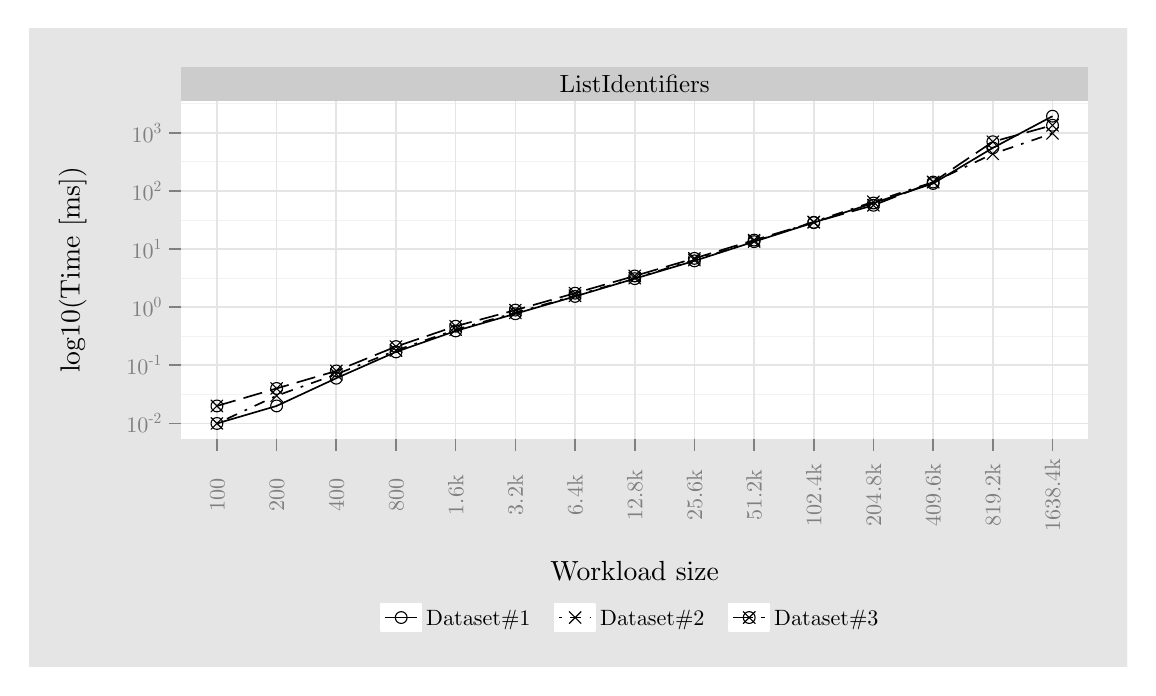
\begin{tikzpicture}[x=1pt,y=1pt]
\definecolor[named]{fillColor}{rgb}{1.00,1.00,1.00}
\path[use as bounding box,fill=fillColor,fill opacity=0.00] (0,0) rectangle (397.48,231.26);
\begin{scope}
\path[clip] (  0.00,  0.00) rectangle (397.48,231.26);
\definecolor[named]{drawColor}{rgb}{1.00,1.00,1.00}
\definecolor[named]{fillColor}{rgb}{0.90,0.90,0.90}

\path[draw=drawColor,line width= 0.6pt,line join=round,line cap=round,fill=fillColor] (  0.00,  0.00) rectangle (397.48,231.26);
\end{scope}
\begin{scope}
\path[clip] ( 55.45, 82.69) rectangle (383.26,204.82);
\definecolor[named]{fillColor}{rgb}{1.00,1.00,1.00}

\path[fill=fillColor] ( 55.45, 82.69) rectangle (383.26,204.82);
\definecolor[named]{drawColor}{rgb}{0.95,0.95,0.95}

\path[draw=drawColor,line width= 0.3pt,line join=round] ( 55.45, 98.75) --
	(383.26, 98.75);

\path[draw=drawColor,line width= 0.3pt,line join=round] ( 55.45,119.76) --
	(383.26,119.76);

\path[draw=drawColor,line width= 0.3pt,line join=round] ( 55.45,140.77) --
	(383.26,140.77);

\path[draw=drawColor,line width= 0.3pt,line join=round] ( 55.45,161.78) --
	(383.26,161.78);

\path[draw=drawColor,line width= 0.3pt,line join=round] ( 55.45,182.79) --
	(383.26,182.79);

\path[draw=drawColor,line width= 0.3pt,line join=round] ( 55.45,203.80) --
	(383.26,203.80);
\definecolor[named]{drawColor}{rgb}{0.90,0.90,0.90}

\path[draw=drawColor,line width= 0.6pt,line join=round] ( 55.45, 88.24) --
	(383.26, 88.24);

\path[draw=drawColor,line width= 0.6pt,line join=round] ( 55.45,109.25) --
	(383.26,109.25);

\path[draw=drawColor,line width= 0.6pt,line join=round] ( 55.45,130.26) --
	(383.26,130.26);

\path[draw=drawColor,line width= 0.6pt,line join=round] ( 55.45,151.28) --
	(383.26,151.28);

\path[draw=drawColor,line width= 0.6pt,line join=round] ( 55.45,172.29) --
	(383.26,172.29);

\path[draw=drawColor,line width= 0.6pt,line join=round] ( 55.45,193.30) --
	(383.26,193.30);

\path[draw=drawColor,line width= 0.6pt,line join=round] ( 68.39, 82.69) --
	( 68.39,204.82);

\path[draw=drawColor,line width= 0.6pt,line join=round] ( 89.95, 82.69) --
	( 89.95,204.82);

\path[draw=drawColor,line width= 0.6pt,line join=round] (111.52, 82.69) --
	(111.52,204.82);

\path[draw=drawColor,line width= 0.6pt,line join=round] (133.09, 82.69) --
	(133.09,204.82);

\path[draw=drawColor,line width= 0.6pt,line join=round] (154.65, 82.69) --
	(154.65,204.82);

\path[draw=drawColor,line width= 0.6pt,line join=round] (176.22, 82.69) --
	(176.22,204.82);

\path[draw=drawColor,line width= 0.6pt,line join=round] (197.79, 82.69) --
	(197.79,204.82);

\path[draw=drawColor,line width= 0.6pt,line join=round] (219.35, 82.69) --
	(219.35,204.82);

\path[draw=drawColor,line width= 0.6pt,line join=round] (240.92, 82.69) --
	(240.92,204.82);

\path[draw=drawColor,line width= 0.6pt,line join=round] (262.49, 82.69) --
	(262.49,204.82);

\path[draw=drawColor,line width= 0.6pt,line join=round] (284.05, 82.69) --
	(284.05,204.82);

\path[draw=drawColor,line width= 0.6pt,line join=round] (305.62, 82.69) --
	(305.62,204.82);

\path[draw=drawColor,line width= 0.6pt,line join=round] (327.19, 82.69) --
	(327.19,204.82);

\path[draw=drawColor,line width= 0.6pt,line join=round] (348.75, 82.69) --
	(348.75,204.82);

\path[draw=drawColor,line width= 0.6pt,line join=round] (370.32, 82.69) --
	(370.32,204.82);
\definecolor[named]{drawColor}{rgb}{0.00,0.00,0.00}

\path[draw=drawColor,line width= 0.6pt,line join=round] ( 68.39, 88.24) --
	( 89.95, 94.57) --
	(111.52,104.59) --
	(133.09,114.10) --
	(154.65,121.67) --
	(176.22,127.88) --
	(197.79,134.15) --
	(219.35,140.56) --
	(240.92,146.99) --
	(262.49,153.93) --
	(284.05,160.82) --
	(305.62,167.90) --
	(327.19,174.95) --
	(348.75,187.81) --
	(370.32,199.27);

\path[draw=drawColor,line width= 0.6pt,dash pattern=on 1pt off 3pt on 4pt off 3pt ,line join=round] ( 68.39, 88.24) --
	( 89.95, 98.27) --
	(111.52,106.00) --
	(133.09,114.62) --
	(154.65,122.13) --
	(176.22,128.23) --
	(197.79,134.38) --
	(219.35,140.76) --
	(240.92,147.30) --
	(262.49,153.98) --
	(284.05,161.11) --
	(305.62,168.35) --
	(327.19,175.45) --
	(348.75,185.65) --
	(370.32,193.06);

\path[draw=drawColor,line width= 0.6pt,dash pattern=on 7pt off 3pt ,line join=round] ( 68.39, 94.57) --
	( 89.95,100.89) --
	(111.52,107.22) --
	(133.09,116.02) --
	(154.65,123.38) --
	(176.22,129.20) --
	(197.79,135.32) --
	(219.35,141.54) --
	(240.92,147.89) --
	(262.49,154.50) --
	(284.05,160.92) --
	(305.62,167.08) --
	(327.19,175.48) --
	(348.75,190.04) --
	(370.32,195.99);

\path[draw=drawColor,line width= 0.4pt,line join=round,line cap=round] ( 68.39, 88.24) circle (  2.13);

\path[draw=drawColor,line width= 0.4pt,line join=round,line cap=round] ( 89.95, 94.57) circle (  2.13);

\path[draw=drawColor,line width= 0.4pt,line join=round,line cap=round] (111.52,104.59) circle (  2.13);

\path[draw=drawColor,line width= 0.4pt,line join=round,line cap=round] (133.09,114.10) circle (  2.13);

\path[draw=drawColor,line width= 0.4pt,line join=round,line cap=round] (154.65,121.67) circle (  2.13);

\path[draw=drawColor,line width= 0.4pt,line join=round,line cap=round] (176.22,127.88) circle (  2.13);

\path[draw=drawColor,line width= 0.4pt,line join=round,line cap=round] (197.79,134.15) circle (  2.13);

\path[draw=drawColor,line width= 0.4pt,line join=round,line cap=round] (219.35,140.56) circle (  2.13);

\path[draw=drawColor,line width= 0.4pt,line join=round,line cap=round] (240.92,146.99) circle (  2.13);

\path[draw=drawColor,line width= 0.4pt,line join=round,line cap=round] (262.49,153.93) circle (  2.13);

\path[draw=drawColor,line width= 0.4pt,line join=round,line cap=round] (284.05,160.82) circle (  2.13);

\path[draw=drawColor,line width= 0.4pt,line join=round,line cap=round] (305.62,167.90) circle (  2.13);

\path[draw=drawColor,line width= 0.4pt,line join=round,line cap=round] (327.19,174.95) circle (  2.13);

\path[draw=drawColor,line width= 0.4pt,line join=round,line cap=round] (348.75,187.81) circle (  2.13);

\path[draw=drawColor,line width= 0.4pt,line join=round,line cap=round] (370.32,199.27) circle (  2.13);

\path[draw=drawColor,line width= 0.4pt,line join=round,line cap=round] ( 68.39, 94.57) circle (  2.13);

\path[draw=drawColor,line width= 0.4pt,line join=round,line cap=round] ( 66.25, 92.43) -- ( 70.52, 96.70);

\path[draw=drawColor,line width= 0.4pt,line join=round,line cap=round] ( 66.25, 96.70) -- ( 70.52, 92.43);

\path[draw=drawColor,line width= 0.4pt,line join=round,line cap=round] ( 89.95,100.89) circle (  2.13);

\path[draw=drawColor,line width= 0.4pt,line join=round,line cap=round] ( 87.82, 98.76) -- ( 92.09,103.03);

\path[draw=drawColor,line width= 0.4pt,line join=round,line cap=round] ( 87.82,103.03) -- ( 92.09, 98.76);

\path[draw=drawColor,line width= 0.4pt,line join=round,line cap=round] (111.52,107.22) circle (  2.13);

\path[draw=drawColor,line width= 0.4pt,line join=round,line cap=round] (109.39,105.08) -- (113.66,109.35);

\path[draw=drawColor,line width= 0.4pt,line join=round,line cap=round] (109.39,109.35) -- (113.66,105.08);

\path[draw=drawColor,line width= 0.4pt,line join=round,line cap=round] (133.09,116.02) circle (  2.13);

\path[draw=drawColor,line width= 0.4pt,line join=round,line cap=round] (130.95,113.89) -- (135.22,118.16);

\path[draw=drawColor,line width= 0.4pt,line join=round,line cap=round] (130.95,118.16) -- (135.22,113.89);

\path[draw=drawColor,line width= 0.4pt,line join=round,line cap=round] (154.65,123.38) circle (  2.13);

\path[draw=drawColor,line width= 0.4pt,line join=round,line cap=round] (152.52,121.24) -- (156.79,125.51);

\path[draw=drawColor,line width= 0.4pt,line join=round,line cap=round] (152.52,125.51) -- (156.79,121.24);

\path[draw=drawColor,line width= 0.4pt,line join=round,line cap=round] (176.22,129.20) circle (  2.13);

\path[draw=drawColor,line width= 0.4pt,line join=round,line cap=round] (174.09,127.07) -- (178.35,131.34);

\path[draw=drawColor,line width= 0.4pt,line join=round,line cap=round] (174.09,131.34) -- (178.35,127.07);

\path[draw=drawColor,line width= 0.4pt,line join=round,line cap=round] (197.79,135.32) circle (  2.13);

\path[draw=drawColor,line width= 0.4pt,line join=round,line cap=round] (195.65,133.19) -- (199.92,137.45);

\path[draw=drawColor,line width= 0.4pt,line join=round,line cap=round] (195.65,137.45) -- (199.92,133.19);

\path[draw=drawColor,line width= 0.4pt,line join=round,line cap=round] (219.35,141.54) circle (  2.13);

\path[draw=drawColor,line width= 0.4pt,line join=round,line cap=round] (217.22,139.40) -- (221.49,143.67);

\path[draw=drawColor,line width= 0.4pt,line join=round,line cap=round] (217.22,143.67) -- (221.49,139.40);

\path[draw=drawColor,line width= 0.4pt,line join=round,line cap=round] (240.92,147.89) circle (  2.13);

\path[draw=drawColor,line width= 0.4pt,line join=round,line cap=round] (238.79,145.76) -- (243.05,150.02);

\path[draw=drawColor,line width= 0.4pt,line join=round,line cap=round] (238.79,150.02) -- (243.05,145.76);

\path[draw=drawColor,line width= 0.4pt,line join=round,line cap=round] (262.49,154.50) circle (  2.13);

\path[draw=drawColor,line width= 0.4pt,line join=round,line cap=round] (260.35,152.36) -- (264.62,156.63);

\path[draw=drawColor,line width= 0.4pt,line join=round,line cap=round] (260.35,156.63) -- (264.62,152.36);

\path[draw=drawColor,line width= 0.4pt,line join=round,line cap=round] (284.05,160.92) circle (  2.13);

\path[draw=drawColor,line width= 0.4pt,line join=round,line cap=round] (281.92,158.79) -- (286.19,163.05);

\path[draw=drawColor,line width= 0.4pt,line join=round,line cap=round] (281.92,163.05) -- (286.19,158.79);

\path[draw=drawColor,line width= 0.4pt,line join=round,line cap=round] (305.62,167.08) circle (  2.13);

\path[draw=drawColor,line width= 0.4pt,line join=round,line cap=round] (303.49,164.95) -- (307.75,169.21);

\path[draw=drawColor,line width= 0.4pt,line join=round,line cap=round] (303.49,169.21) -- (307.75,164.95);

\path[draw=drawColor,line width= 0.4pt,line join=round,line cap=round] (327.19,175.48) circle (  2.13);

\path[draw=drawColor,line width= 0.4pt,line join=round,line cap=round] (325.05,173.35) -- (329.32,177.62);

\path[draw=drawColor,line width= 0.4pt,line join=round,line cap=round] (325.05,177.62) -- (329.32,173.35);

\path[draw=drawColor,line width= 0.4pt,line join=round,line cap=round] (348.75,190.04) circle (  2.13);

\path[draw=drawColor,line width= 0.4pt,line join=round,line cap=round] (346.62,187.91) -- (350.89,192.18);

\path[draw=drawColor,line width= 0.4pt,line join=round,line cap=round] (346.62,192.18) -- (350.89,187.91);

\path[draw=drawColor,line width= 0.4pt,line join=round,line cap=round] (370.32,195.99) circle (  2.13);

\path[draw=drawColor,line width= 0.4pt,line join=round,line cap=round] (368.18,193.85) -- (372.45,198.12);

\path[draw=drawColor,line width= 0.4pt,line join=round,line cap=round] (368.18,198.12) -- (372.45,193.85);

\path[draw=drawColor,line width= 0.4pt,line join=round,line cap=round,fill=fillColor] ( 66.25, 86.11) -- ( 70.52, 90.38);

\path[draw=drawColor,line width= 0.4pt,line join=round,line cap=round,fill=fillColor] ( 66.25, 90.38) -- ( 70.52, 86.11);

\path[draw=drawColor,line width= 0.4pt,line join=round,line cap=round,fill=fillColor] ( 87.82, 96.13) -- ( 92.09,100.40);

\path[draw=drawColor,line width= 0.4pt,line join=round,line cap=round,fill=fillColor] ( 87.82,100.40) -- ( 92.09, 96.13);

\path[draw=drawColor,line width= 0.4pt,line join=round,line cap=round,fill=fillColor] (109.39,103.86) -- (113.66,108.13);

\path[draw=drawColor,line width= 0.4pt,line join=round,line cap=round,fill=fillColor] (109.39,108.13) -- (113.66,103.86);

\path[draw=drawColor,line width= 0.4pt,line join=round,line cap=round,fill=fillColor] (130.95,112.48) -- (135.22,116.75);

\path[draw=drawColor,line width= 0.4pt,line join=round,line cap=round,fill=fillColor] (130.95,116.75) -- (135.22,112.48);

\path[draw=drawColor,line width= 0.4pt,line join=round,line cap=round,fill=fillColor] (152.52,119.99) -- (156.79,124.26);

\path[draw=drawColor,line width= 0.4pt,line join=round,line cap=round,fill=fillColor] (152.52,124.26) -- (156.79,119.99);

\path[draw=drawColor,line width= 0.4pt,line join=round,line cap=round,fill=fillColor] (174.09,126.09) -- (178.35,130.36);

\path[draw=drawColor,line width= 0.4pt,line join=round,line cap=round,fill=fillColor] (174.09,130.36) -- (178.35,126.09);

\path[draw=drawColor,line width= 0.4pt,line join=round,line cap=round,fill=fillColor] (195.65,132.25) -- (199.92,136.51);

\path[draw=drawColor,line width= 0.4pt,line join=round,line cap=round,fill=fillColor] (195.65,136.51) -- (199.92,132.25);

\path[draw=drawColor,line width= 0.4pt,line join=round,line cap=round,fill=fillColor] (217.22,138.63) -- (221.49,142.90);

\path[draw=drawColor,line width= 0.4pt,line join=round,line cap=round,fill=fillColor] (217.22,142.90) -- (221.49,138.63);

\path[draw=drawColor,line width= 0.4pt,line join=round,line cap=round,fill=fillColor] (238.79,145.17) -- (243.05,149.44);

\path[draw=drawColor,line width= 0.4pt,line join=round,line cap=round,fill=fillColor] (238.79,149.44) -- (243.05,145.17);

\path[draw=drawColor,line width= 0.4pt,line join=round,line cap=round,fill=fillColor] (260.35,151.85) -- (264.62,156.11);

\path[draw=drawColor,line width= 0.4pt,line join=round,line cap=round,fill=fillColor] (260.35,156.11) -- (264.62,151.85);

\path[draw=drawColor,line width= 0.4pt,line join=round,line cap=round,fill=fillColor] (281.92,158.97) -- (286.19,163.24);

\path[draw=drawColor,line width= 0.4pt,line join=round,line cap=round,fill=fillColor] (281.92,163.24) -- (286.19,158.97);

\path[draw=drawColor,line width= 0.4pt,line join=round,line cap=round,fill=fillColor] (303.49,166.21) -- (307.75,170.48);

\path[draw=drawColor,line width= 0.4pt,line join=round,line cap=round,fill=fillColor] (303.49,170.48) -- (307.75,166.21);

\path[draw=drawColor,line width= 0.4pt,line join=round,line cap=round,fill=fillColor] (325.05,173.32) -- (329.32,177.59);

\path[draw=drawColor,line width= 0.4pt,line join=round,line cap=round,fill=fillColor] (325.05,177.59) -- (329.32,173.32);

\path[draw=drawColor,line width= 0.4pt,line join=round,line cap=round,fill=fillColor] (346.62,183.52) -- (350.89,187.79);

\path[draw=drawColor,line width= 0.4pt,line join=round,line cap=round,fill=fillColor] (346.62,187.79) -- (350.89,183.52);

\path[draw=drawColor,line width= 0.4pt,line join=round,line cap=round,fill=fillColor] (368.18,190.92) -- (372.45,195.19);

\path[draw=drawColor,line width= 0.4pt,line join=round,line cap=round,fill=fillColor] (368.18,195.19) -- (372.45,190.92);
\end{scope}
\begin{scope}
\path[clip] (  0.00,  0.00) rectangle (397.48,231.26);
\definecolor[named]{fillColor}{rgb}{0.80,0.80,0.80}

\path[fill=fillColor] ( 55.45,204.82) rectangle (383.26,217.04);
\definecolor[named]{drawColor}{rgb}{0.00,0.00,0.00}

\node[text=drawColor,anchor=base,inner sep=0pt, outer sep=0pt, scale=  0.90] at (219.35,207.83) {ListIdentifiers};
\end{scope}
\begin{scope}
\path[clip] (  0.00,  0.00) rectangle (397.48,231.26);
\definecolor[named]{drawColor}{rgb}{0.50,0.50,0.50}

\node[text=drawColor,anchor=base west,inner sep=0pt, outer sep=0pt, scale=  0.80] at ( 35.67, 84.81) {10};

\node[text=drawColor,anchor=base west,inner sep=0pt, outer sep=0pt, scale=  0.56] at ( 43.67, 88.08) {-};

\node[text=drawColor,anchor=base west,inner sep=0pt, outer sep=0pt, scale=  0.56] at ( 45.54, 88.08) {2};

\node[text=drawColor,anchor=base west,inner sep=0pt, outer sep=0pt, scale=  0.80] at ( 35.67,105.82) {10};

\node[text=drawColor,anchor=base west,inner sep=0pt, outer sep=0pt, scale=  0.56] at ( 43.67,109.09) {-};

\node[text=drawColor,anchor=base west,inner sep=0pt, outer sep=0pt, scale=  0.56] at ( 45.54,109.09) {1};

\node[text=drawColor,anchor=base west,inner sep=0pt, outer sep=0pt, scale=  0.80] at ( 37.54,126.83) {10};

\node[text=drawColor,anchor=base west,inner sep=0pt, outer sep=0pt, scale=  0.56] at ( 45.54,130.10) {0};

\node[text=drawColor,anchor=base west,inner sep=0pt, outer sep=0pt, scale=  0.80] at ( 37.54,147.84) {10};

\node[text=drawColor,anchor=base west,inner sep=0pt, outer sep=0pt, scale=  0.56] at ( 45.54,151.12) {1};

\node[text=drawColor,anchor=base west,inner sep=0pt, outer sep=0pt, scale=  0.80] at ( 37.54,168.86) {10};

\node[text=drawColor,anchor=base west,inner sep=0pt, outer sep=0pt, scale=  0.56] at ( 45.54,172.13) {2};

\node[text=drawColor,anchor=base west,inner sep=0pt, outer sep=0pt, scale=  0.80] at ( 37.54,189.87) {10};

\node[text=drawColor,anchor=base west,inner sep=0pt, outer sep=0pt, scale=  0.56] at ( 45.54,193.14) {3};
\end{scope}
\begin{scope}
\path[clip] (  0.00,  0.00) rectangle (397.48,231.26);
\definecolor[named]{drawColor}{rgb}{0.50,0.50,0.50}

\path[draw=drawColor,line width= 0.6pt,line join=round] ( 51.18, 88.24) --
	( 55.45, 88.24);

\path[draw=drawColor,line width= 0.6pt,line join=round] ( 51.18,109.25) --
	( 55.45,109.25);

\path[draw=drawColor,line width= 0.6pt,line join=round] ( 51.18,130.26) --
	( 55.45,130.26);

\path[draw=drawColor,line width= 0.6pt,line join=round] ( 51.18,151.28) --
	( 55.45,151.28);

\path[draw=drawColor,line width= 0.6pt,line join=round] ( 51.18,172.29) --
	( 55.45,172.29);

\path[draw=drawColor,line width= 0.6pt,line join=round] ( 51.18,193.30) --
	( 55.45,193.30);
\end{scope}
\begin{scope}
\path[clip] (  0.00,  0.00) rectangle (397.48,231.26);
\definecolor[named]{drawColor}{rgb}{0.50,0.50,0.50}

\path[draw=drawColor,line width= 0.6pt,line join=round] ( 68.39, 78.42) --
	( 68.39, 82.69);

\path[draw=drawColor,line width= 0.6pt,line join=round] ( 89.95, 78.42) --
	( 89.95, 82.69);

\path[draw=drawColor,line width= 0.6pt,line join=round] (111.52, 78.42) --
	(111.52, 82.69);

\path[draw=drawColor,line width= 0.6pt,line join=round] (133.09, 78.42) --
	(133.09, 82.69);

\path[draw=drawColor,line width= 0.6pt,line join=round] (154.65, 78.42) --
	(154.65, 82.69);

\path[draw=drawColor,line width= 0.6pt,line join=round] (176.22, 78.42) --
	(176.22, 82.69);

\path[draw=drawColor,line width= 0.6pt,line join=round] (197.79, 78.42) --
	(197.79, 82.69);

\path[draw=drawColor,line width= 0.6pt,line join=round] (219.35, 78.42) --
	(219.35, 82.69);

\path[draw=drawColor,line width= 0.6pt,line join=round] (240.92, 78.42) --
	(240.92, 82.69);

\path[draw=drawColor,line width= 0.6pt,line join=round] (262.49, 78.42) --
	(262.49, 82.69);

\path[draw=drawColor,line width= 0.6pt,line join=round] (284.05, 78.42) --
	(284.05, 82.69);

\path[draw=drawColor,line width= 0.6pt,line join=round] (305.62, 78.42) --
	(305.62, 82.69);

\path[draw=drawColor,line width= 0.6pt,line join=round] (327.19, 78.42) --
	(327.19, 82.69);

\path[draw=drawColor,line width= 0.6pt,line join=round] (348.75, 78.42) --
	(348.75, 82.69);

\path[draw=drawColor,line width= 0.6pt,line join=round] (370.32, 78.42) --
	(370.32, 82.69);
\end{scope}
\begin{scope}
\path[clip] (  0.00,  0.00) rectangle (397.48,231.26);
\definecolor[named]{drawColor}{rgb}{0.50,0.50,0.50}

\node[text=drawColor,rotate= 90.00,anchor=base,inner sep=0pt, outer sep=0pt, scale=  0.80] at ( 71.14, 62.36) {100};

\node[text=drawColor,rotate= 90.00,anchor=base,inner sep=0pt, outer sep=0pt, scale=  0.80] at ( 92.71, 62.36) {200};

\node[text=drawColor,rotate= 90.00,anchor=base,inner sep=0pt, outer sep=0pt, scale=  0.80] at (114.28, 62.36) {400};

\node[text=drawColor,rotate= 90.00,anchor=base,inner sep=0pt, outer sep=0pt, scale=  0.80] at (135.84, 62.36) {800};

\node[text=drawColor,rotate= 90.00,anchor=base,inner sep=0pt, outer sep=0pt, scale=  0.80] at (157.41, 62.36) {1.6k};

\node[text=drawColor,rotate= 90.00,anchor=base,inner sep=0pt, outer sep=0pt, scale=  0.80] at (178.98, 62.36) {3.2k};

\node[text=drawColor,rotate= 90.00,anchor=base,inner sep=0pt, outer sep=0pt, scale=  0.80] at (200.54, 62.36) {6.4k};

\node[text=drawColor,rotate= 90.00,anchor=base,inner sep=0pt, outer sep=0pt, scale=  0.80] at (222.11, 62.36) {12.8k};

\node[text=drawColor,rotate= 90.00,anchor=base,inner sep=0pt, outer sep=0pt, scale=  0.80] at (243.67, 62.36) {25.6k};

\node[text=drawColor,rotate= 90.00,anchor=base,inner sep=0pt, outer sep=0pt, scale=  0.80] at (265.24, 62.36) {51.2k};

\node[text=drawColor,rotate= 90.00,anchor=base,inner sep=0pt, outer sep=0pt, scale=  0.80] at (286.81, 62.36) {102.4k};

\node[text=drawColor,rotate= 90.00,anchor=base,inner sep=0pt, outer sep=0pt, scale=  0.80] at (308.37, 62.36) {204.8k};

\node[text=drawColor,rotate= 90.00,anchor=base,inner sep=0pt, outer sep=0pt, scale=  0.80] at (329.94, 62.36) {409.6k};

\node[text=drawColor,rotate= 90.00,anchor=base,inner sep=0pt, outer sep=0pt, scale=  0.80] at (351.51, 62.36) {819.2k};

\node[text=drawColor,rotate= 90.00,anchor=base,inner sep=0pt, outer sep=0pt, scale=  0.80] at (373.07, 62.36) {1638.4k};
\end{scope}
\begin{scope}
\path[clip] (  0.00,  0.00) rectangle (397.48,231.26);
\definecolor[named]{drawColor}{rgb}{0.00,0.00,0.00}

\node[text=drawColor,anchor=base,inner sep=0pt, outer sep=0pt, scale=  1.00] at (219.35, 31.41) {Workload size};
\end{scope}
\begin{scope}
\path[clip] (  0.00,  0.00) rectangle (397.48,231.26);
\definecolor[named]{drawColor}{rgb}{0.00,0.00,0.00}

\node[text=drawColor,rotate= 90.00,anchor=base,inner sep=0pt, outer sep=0pt, scale=  1.00] at ( 18.80,143.75) {log10(Time [ms])};
\end{scope}
\begin{scope}
\path[clip] (  0.00,  0.00) rectangle (397.48,231.26);
\definecolor[named]{fillColor}{rgb}{0.90,0.90,0.90}

\path[fill=fillColor] (119.86,  8.87) rectangle (318.84, 27.36);
\end{scope}
\begin{scope}
\path[clip] (  0.00,  0.00) rectangle (397.48,231.26);
\definecolor[named]{drawColor}{rgb}{1.00,1.00,1.00}
\definecolor[named]{fillColor}{rgb}{1.00,1.00,1.00}

\path[draw=drawColor,line width= 0.6pt,line join=round,line cap=round,fill=fillColor] (127.74, 13.14) rectangle (142.20, 23.09);
\end{scope}
\begin{scope}
\path[clip] (  0.00,  0.00) rectangle (397.48,231.26);
\definecolor[named]{drawColor}{rgb}{0.00,0.00,0.00}

\path[draw=drawColor,line width= 0.6pt,line join=round] (129.19, 18.11) -- (140.75, 18.11);
\end{scope}
\begin{scope}
\path[clip] (  0.00,  0.00) rectangle (397.48,231.26);
\definecolor[named]{drawColor}{rgb}{0.00,0.00,0.00}

\path[draw=drawColor,line width= 0.4pt,line join=round,line cap=round] (134.97, 18.11) circle (  2.13);
\end{scope}
\begin{scope}
\path[clip] (  0.00,  0.00) rectangle (397.48,231.26);
\definecolor[named]{drawColor}{rgb}{1.00,1.00,1.00}
\definecolor[named]{fillColor}{rgb}{1.00,1.00,1.00}

\path[draw=drawColor,line width= 0.6pt,line join=round,line cap=round,fill=fillColor] (190.62, 13.14) rectangle (205.08, 23.09);
\end{scope}
\begin{scope}
\path[clip] (  0.00,  0.00) rectangle (397.48,231.26);
\definecolor[named]{drawColor}{rgb}{0.00,0.00,0.00}

\path[draw=drawColor,line width= 0.6pt,dash pattern=on 1pt off 3pt on 4pt off 3pt ,line join=round] (192.07, 18.11) -- (203.63, 18.11);
\end{scope}
\begin{scope}
\path[clip] (  0.00,  0.00) rectangle (397.48,231.26);
\definecolor[named]{drawColor}{rgb}{0.00,0.00,0.00}
\definecolor[named]{fillColor}{rgb}{1.00,1.00,1.00}

\path[draw=drawColor,line width= 0.4pt,line join=round,line cap=round,fill=fillColor] (195.72, 15.98) -- (199.98, 20.25);

\path[draw=drawColor,line width= 0.4pt,line join=round,line cap=round,fill=fillColor] (195.72, 20.25) -- (199.98, 15.98);
\end{scope}
\begin{scope}
\path[clip] (  0.00,  0.00) rectangle (397.48,231.26);
\definecolor[named]{drawColor}{rgb}{1.00,1.00,1.00}
\definecolor[named]{fillColor}{rgb}{1.00,1.00,1.00}

\path[draw=drawColor,line width= 0.6pt,line join=round,line cap=round,fill=fillColor] (253.50, 13.14) rectangle (267.96, 23.09);
\end{scope}
\begin{scope}
\path[clip] (  0.00,  0.00) rectangle (397.48,231.26);
\definecolor[named]{drawColor}{rgb}{0.00,0.00,0.00}

\path[draw=drawColor,line width= 0.6pt,dash pattern=on 7pt off 3pt ,line join=round] (254.95, 18.11) -- (266.51, 18.11);
\end{scope}
\begin{scope}
\path[clip] (  0.00,  0.00) rectangle (397.48,231.26);
\definecolor[named]{drawColor}{rgb}{0.00,0.00,0.00}

\path[draw=drawColor,line width= 0.4pt,line join=round,line cap=round] (260.73, 18.11) circle (  2.13);

\path[draw=drawColor,line width= 0.4pt,line join=round,line cap=round] (258.60, 15.98) -- (262.86, 20.25);

\path[draw=drawColor,line width= 0.4pt,line join=round,line cap=round] (258.60, 20.25) -- (262.86, 15.98);
\end{scope}
\begin{scope}
\path[clip] (  0.00,  0.00) rectangle (397.48,231.26);
\definecolor[named]{drawColor}{rgb}{0.00,0.00,0.00}

\node[text=drawColor,anchor=base west,inner sep=0pt, outer sep=0pt, scale=  0.80] at (144.00, 15.36) {Dataset\#1 $\;\;$};
\end{scope}
\begin{scope}
\path[clip] (  0.00,  0.00) rectangle (397.48,231.26);
\definecolor[named]{drawColor}{rgb}{0.00,0.00,0.00}

\node[text=drawColor,anchor=base west,inner sep=0pt, outer sep=0pt, scale=  0.80] at (206.88, 15.36) {Dataset\#2 $\;\;$};
\end{scope}
\begin{scope}
\path[clip] (  0.00,  0.00) rectangle (397.48,231.26);
\definecolor[named]{drawColor}{rgb}{0.00,0.00,0.00}

\node[text=drawColor,anchor=base west,inner sep=0pt, outer sep=0pt, scale=  0.80] at (269.76, 15.36) {Dataset\#3 $\;\;$};
\end{scope}
\end{tikzpicture}
